\documentclass[10pt, a4paper]{beamer}
\usepackage{multirow}

\usepackage[english]{babel}
\usepackage{blindtext}

\usepackage{graphicx}
\usepackage[export]{adjustbox}
\usepackage{wrapfig}

\usetheme{Berkeley}
\usecolortheme{sidebartab}

\newcommand\tab[1][1cm]{\hspace*{#1}}
\newcommand\tabhalf[1][0.5cm]{\hspace*{#1}}

\begin{document}
	\setbeamertemplate{sidebar left}{}
	\title{Progress Presentation-II}
	\subtitle{e-Yantra Summer Internship-2018 \\Machine Learning and It's Application}
	\author{Swapnil Masurekar\\Abhishek Sharma\\
	Mentors: Rutuja, Suprabha}
	\institute{IIT Bombay}
	\date{\today}
	%\addtobeamertemplate{sidebar left}{}{\includegraphics[scale = 0.3]{logowithtext.png}}
	\frame{\titlepage}

\setbeamertemplate{sidebar left}[sidebar theme]
\section{Overview of Project}
\begin{frame}{Overview of Project}
	
	\begin{itemize}
		\item Project Name : \textbf{Machine Learning and It's Application}\\
		\item Objective : To study machine learning and to work on its practical applications of Character Recognition, Automated Reply, Face Recognition along with documentation\\
		\item Deliverables : 
          \begin{enumerate}
          \item Learning ML and implement Applications
          \item Well commented code and documentation\\ 
          \end{enumerate}
	\end{itemize}
\end{frame}

\section{Overview of Task}
\begin{frame}{Overview of Task}
	\begin{tabular}{| c | l | c |}\hline
    \textbf{Task no.} & \hspace{2.9cm} \textbf{Task}  & \textbf{Status} \\\hline
    \multicolumn{3}{ |c| }{\textbf{Week 1}} \\
    \hline
    1 & Learning Basics of ML& Completed \\\hline
     2 & Get familiar with Tensorflow(and python)    & Completed \\\hline
     
     \multicolumn{3}{ |c| }{\textbf{Week 2}}  \\
     \hline
    
     3 &  Character recognition using LR & Completed \\\hline
     4 & Character recognition using neural network & Completed \\\hline
     
     \multicolumn{3}{ |c| }{\textbf{Week 3 and Week 4}} \\
     \hline
    
     5 &  Automated Reply System & Completed \\\hline
    
     \multicolumn{3}{ |c| }{\textbf{Week 5}} \\
     \hline
         
     6 & Face Recognition & Ongoing \\\hline
     
     \multicolumn{3}{ |c| }{\textbf{Week 6}} \\
     \hline
         
     7 & Documentation & Ongoing   \\\hline
 
    \end{tabular}
    
\end{frame}

\section{Task Accomplished}
\begin{frame}{Improvisations in Character Recognition}
\begin{itemize}
\item Further expanding Dataset with Morphological transformations
\item Sentence detection:
    \begin{figure}
 	    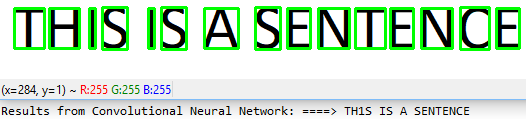
\includegraphics[height=0.27 \textheight]{testSENTENCE.png}
	\end{figure}

\item Dotted Character Recognition:
    \begin{figure}
 	    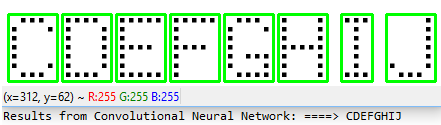
\includegraphics[height=0.27 \textheight]{test_CDEFGHIJ_dotted.png}
	\end{figure}
\end{itemize}
\end{frame}


\begin{frame}{Text Processing}
    \begin{figure}
 	    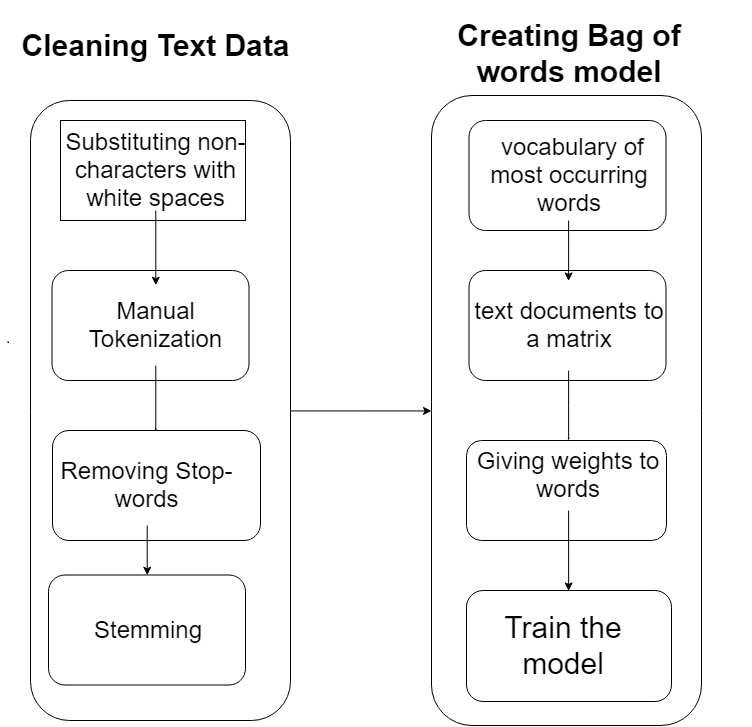
\includegraphics[height=0.90 \textheight]{flowchart_2.png}
	\end{figure}
\end{frame}


\begin{frame}{Automated Reply: Category Classification}
\textbf{Gaussian Naive Bayes}
	\begin{itemize}
		\item To label the mail in gmail inbox
	\end{itemize}
\textbf{Nearest Neighbor}
	\begin{itemize}
		\item To generate the reply for the query
	\end{itemize}
\end{frame}

\begin{frame}{
\includegraphics[width=0.07 \textwidth, right=0.6cm]{google-developers-logo.png}\tabhalf Automatic Mail Labeling using Gmail API}
  \begin{figure}
   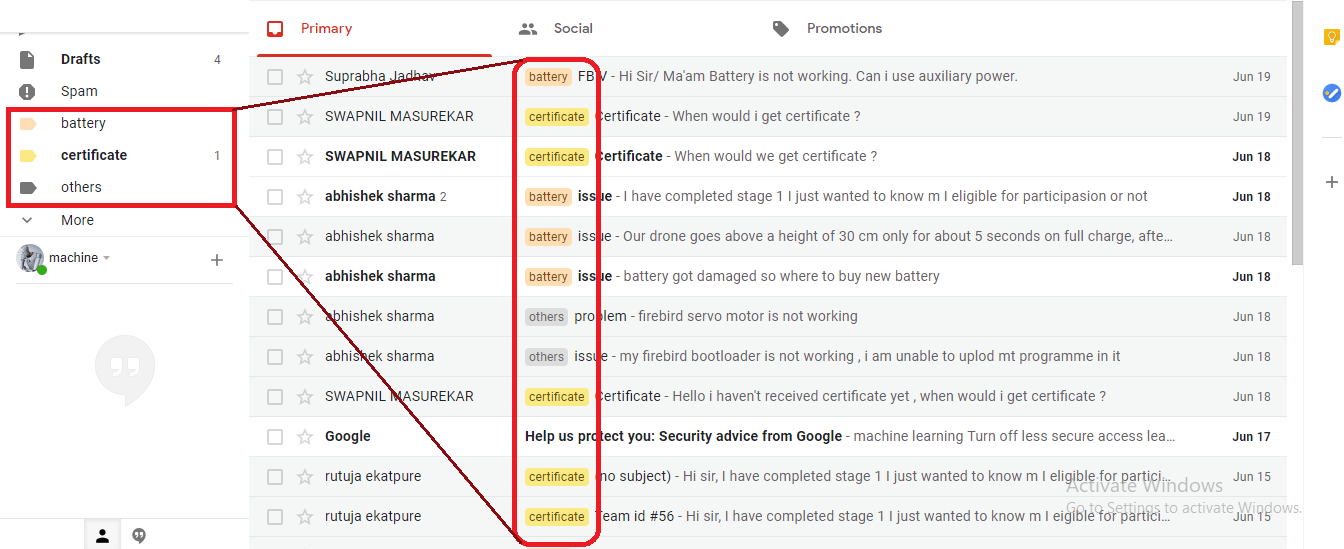
\includegraphics[width=1.13 \textwidth, right=11.1cm]{gmail_labeling.png}
   \caption{Automatic Mail Labeling using Gmail API}
  \end{figure}
\end{frame}

\begin{frame}{
\includegraphics[width=0.07 \textwidth, right=0.6cm]{google-developers-logo.png}\tabhalf Automated Reply to E-mail query}
\begin{columns}
 \column{0.5 \textwidth}
    \begin{figure}
 	    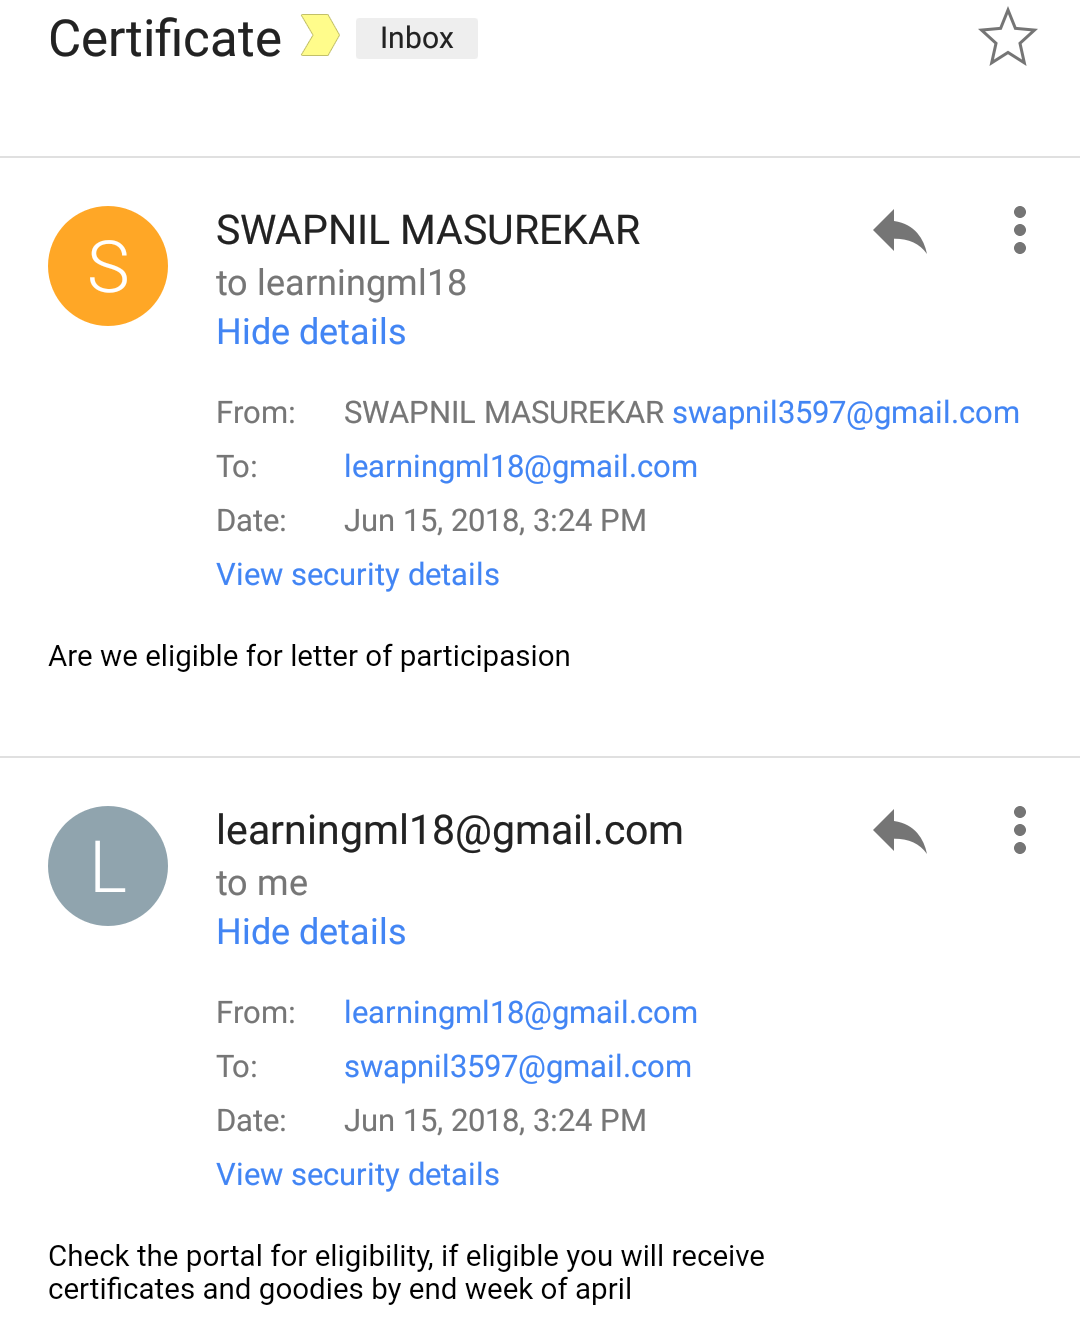
\includegraphics[height=0.8 \textheight]{reply1.png}
	\end{figure}
 \column{0.5 \textwidth}
 \begin{figure}
 	    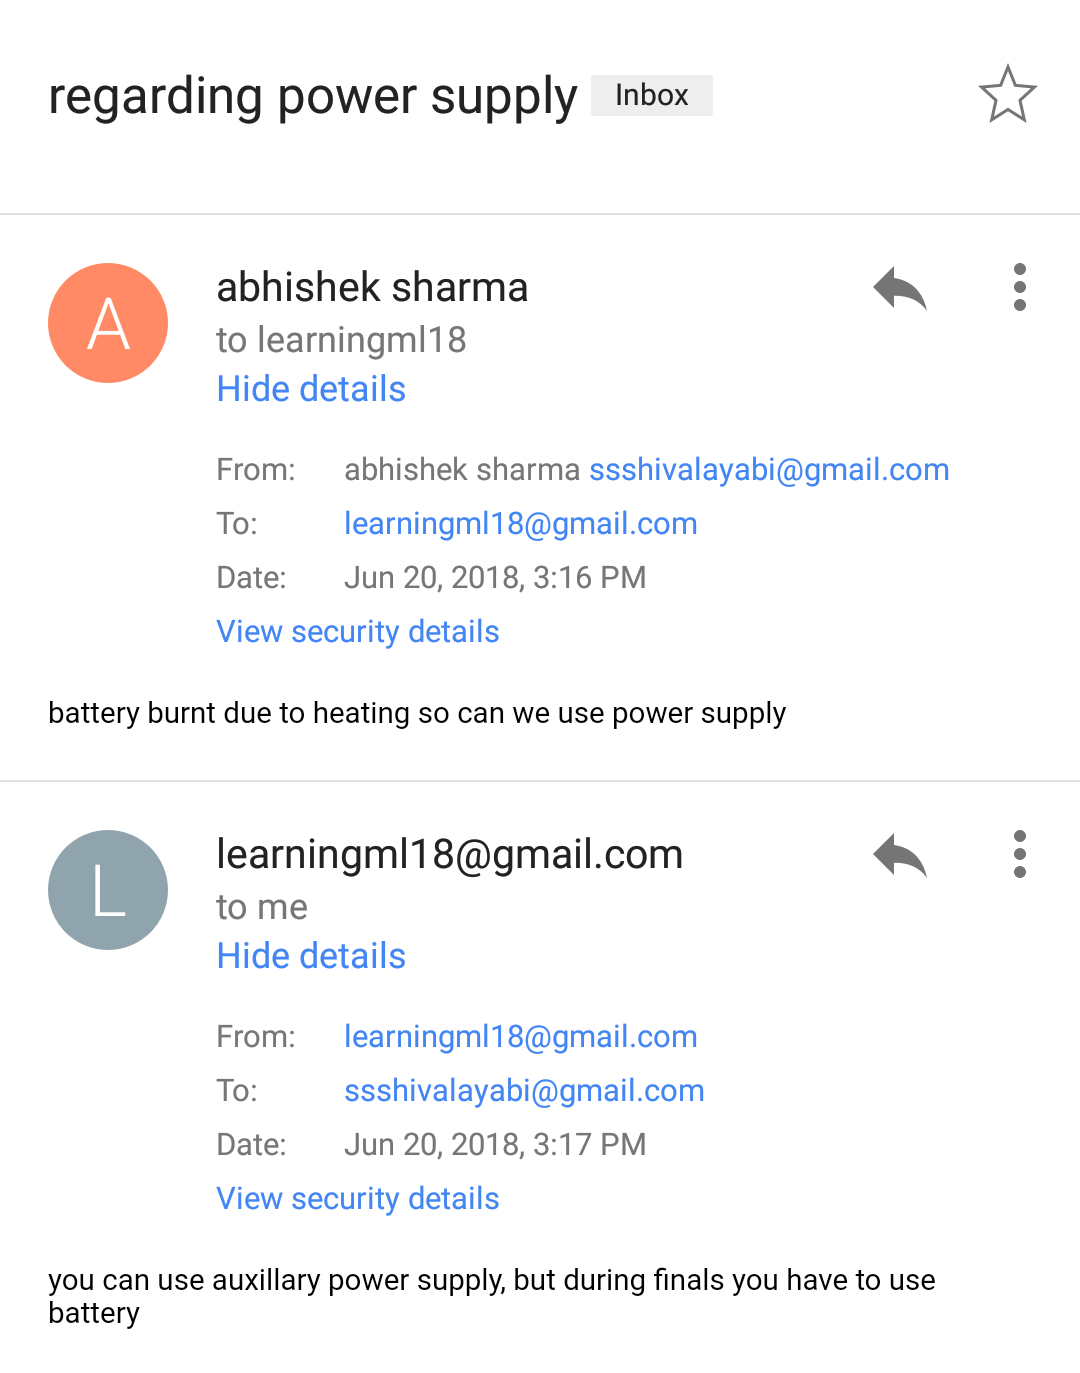
\includegraphics[height=0.8 \textheight]{reply2.png}
	\end{figure}
\end{columns}
\end{frame}


\section{Challenges Faced}
\begin{frame}{Challenges Faced}
	\begin{itemize}
    	\item Word Embeddings (word2vec)
    	\item Finding best approach for finding most similar query to current query from Dataset:
          \begin{enumerate}
          \item Sentence Similarity Based on Semantic Nets
and Corpus Statistics
          \item Using Recurrent Neural Network for sequence classification
          \end{enumerate}
        \item Getting used to Gmail API
        \item Dotted Character Detection
	\end{itemize}
\end{frame}

\section{Future Plans}
\begin{frame}{Future Plans}
	\begin{itemize}
    	\item Optical Character-Recognition:
        \begin{itemize}
        	\item Detection of characters on ruled pages
            \item Improvement in accuracy
        \end{itemize}
		\item Face - Recognition  
	\end{itemize}
\end{frame}


\section{Thank You}
\begin{frame}{Thank You}
	\centering THANK YOU !!!
\end{frame}
\end{document}
